%\VignetteIndexEntry{coMET users guide}
%\VignetteDepends{coMET}
%\VignetteKeywords{Software, Visualization, GenomeAnnotation, GeneRegulation, GenomicVariation, DNAMethylation, SNP, GeneExpression }
%\VignettePackage{coMET}
%\VignetteEngine{knitr::knitr}

\documentclass[11pt]{article}\usepackage[]{graphicx}\usepackage[usenames,dvipsnames]{color}
%% maxwidth is the original width if it is less than linewidth
%% otherwise use linewidth (to make sure the graphics do not exceed the margin)
\makeatletter
\def\maxwidth{ %
  \ifdim\Gin@nat@width>\linewidth
    \linewidth
  \else
    \Gin@nat@width
  \fi
}
\makeatother

\definecolor{fgcolor}{rgb}{0.345, 0.345, 0.345}
\newcommand{\hlnum}[1]{\textcolor[rgb]{0.686,0.059,0.569}{#1}}%
\newcommand{\hlstr}[1]{\textcolor[rgb]{0.192,0.494,0.8}{#1}}%
\newcommand{\hlcom}[1]{\textcolor[rgb]{0.678,0.584,0.686}{\textit{#1}}}%
\newcommand{\hlopt}[1]{\textcolor[rgb]{0,0,0}{#1}}%
\newcommand{\hlstd}[1]{\textcolor[rgb]{0.345,0.345,0.345}{#1}}%
\newcommand{\hlkwa}[1]{\textcolor[rgb]{0.161,0.373,0.58}{\textbf{#1}}}%
\newcommand{\hlkwb}[1]{\textcolor[rgb]{0.69,0.353,0.396}{#1}}%
\newcommand{\hlkwc}[1]{\textcolor[rgb]{0.333,0.667,0.333}{#1}}%
\newcommand{\hlkwd}[1]{\textcolor[rgb]{0.737,0.353,0.396}{\textbf{#1}}}%

\usepackage{framed}
\makeatletter
\newenvironment{kframe}{%
 \def\at@end@of@kframe{}%
 \ifinner\ifhmode%
  \def\at@end@of@kframe{\end{minipage}}%
  \begin{minipage}{\columnwidth}%
 \fi\fi%
 \def\FrameCommand##1{\hskip\@totalleftmargin \hskip-\fboxsep
 \colorbox{shadecolor}{##1}\hskip-\fboxsep
     % There is no \\@totalrightmargin, so:
     \hskip-\linewidth \hskip-\@totalleftmargin \hskip\columnwidth}%
 \MakeFramed {\advance\hsize-\width
   \@totalleftmargin\z@ \linewidth\hsize
   \@setminipage}}%
 {\par\unskip\endMakeFramed%
 \at@end@of@kframe}
\makeatother

\definecolor{shadecolor}{rgb}{.97, .97, .97}
\definecolor{messagecolor}{rgb}{0, 0, 0}
\definecolor{warningcolor}{rgb}{1, 0, 1}
\definecolor{errorcolor}{rgb}{1, 0, 0}
\newenvironment{knitrout}{}{} % an empty environment to be redefined in TeX

\usepackage{alltt}

% A bunch of styles and package requirements for the Bioconductor vignette branding
\RequirePackage{/home/tiphaine/R/x86_64-pc-linux-gnu-library/3.1/BiocStyle/sty/Bioconductor}

\AtBeginDocument{\bibliographystyle{/home/tiphaine/R/x86_64-pc-linux-gnu-library/3.1/BiocStyle/sty/unsrturl}}




\RequirePackage[utf8]{inputenc} 
% \RequirePackage{hyperref}
\RequirePackage{url}
\RequirePackage[authoryear,round]{natbib}
\bibliographystyle{plainnat}
% \RequirePackage[text={7.2in,9in},centering]{geometry}
%\setkeys{Gin}{width=0.95\textwidth}
\RequirePackage{longtable}
\RequirePackage{graphicx}
\newcommand{\code}[1]{{\texttt{#1}}}
\newcommand{\term}[1]{{\emph{#1}}}
\newcommand{\Rmethod}[1]{{\textit{#1}}}
\newcommand{\Rfunarg}[1]{{\textit{#1}}}
\newcommand{\scscst}{\scriptscriptstyle}
\newcommand{\scst}{\scriptstyle}
\newcommand{\mgg}[0]{\Rpackage{coMET} }
\newcommand{\Reference}[1]{{\texttt{#1}}}
\newcommand{\link}[1]{{#1}}
\newcommand{\RR}[0]{{\texttt{R}}}

\title{The coMET User Guide}
\author{Tiphaine Martin \footnote{tiphaine.martin@kcl.ac.uk}, Idil Yet \footnote{idil.yet@kcl.ac.uk}, Pei-Chien Tsai \footnote{peichien.tsai@kcl.ac.uk}, Jordana T. Bell \footnote{jordana.bell@kcl.ac.uk}}
\date{Edited: September 2014; Compiled: \today}
\IfFileExists{upquote.sty}{\usepackage{upquote}}{}
\begin{document}

\maketitle

\section{Citation}
\begin{knitrout}
\definecolor{shadecolor}{rgb}{0.969, 0.969, 0.969}\color{fgcolor}\begin{kframe}
\begin{alltt}
\hlkwd{citation}\hlstd{(}\hlkwc{package}\hlstd{=}\hlstr{'coMET'}\hlstd{)}
\end{alltt}
\begin{verbatim}
## 
## To cite package 'coMET' in publications use:
## 
##   Tiphaine C. Martin, Idil Yet, Pei-Chien Tsai and Jordana T. Bell (2014).
##   coMET: coMET: visualisation of regional epigenome-wide association scan (EWAS)
##   results and DNA co-methylation patterns.. R package version 0.99.3.
##   http://epigen.kcl.ac.uk/comet
## 
## A BibTeX entry for LaTeX users is
## 
##   @Manual{,
##     title = {coMET: coMET: visualisation of regional epigenome-wide association scan (EWAS) results and DNA co-methylation patterns.},
##     author = {Tiphaine C. Martin and Idil Yet and Pei-Chien Tsai and Jordana T. Bell},
##     year = {2014},
##     note = {R package version 0.99.3},
##     url = {http://epigen.kcl.ac.uk/comet},
##   }
## 
## ATTENTION: This citation information has been auto-generated from the package
## DESCRIPTION file and may need manual editing, see 'help("citation")'.
\end{verbatim}
\end{kframe}
\end{knitrout}

\clearpage

\tableofcontents
\clearpage

%%%%%%%%%%%%%%%%%%%%%%%%%%%%%%%%%%%%%%%%%%%%%%%%%%%%%%%%%%%%%%%%%%%%%%%%%%%%%%%
\section{Introduction}
The CoMET package is a web-based plotting tool and R-based package to visualize EWAS (epigenome-wide association scan) results in a genomic region of interest. CoMET provides a plot of the EWAS association signal and visualisation of the methylation correlation between CpG sites (co-methylation). The CoMET package also provides the option to annotate the region using functional genomic information, including both user-defined features and pre-selected features based on the Encode project. The plot can be customized with different parameters, such as plot labels, colours, symbols, heatmap colour scheme, significance thresholds, and including reference CpG sites. Finally, the tool can also be applied to display the correlation patterns of other genomic data, e.g. gene expression array data.

coMET generates a multi-panel plot to visualize EWAS results, co-methylation patterns, and annotation tracks in a genomic region of interest. A coMET figure (cf. Fig. 1) includes three components: 
\begin{enumerate}
  \item the upper plot shows the strength and extent of EWAS association signal;
  \item the middle panel provides customized annotation tracks;
  \item the lower panel shows the correlation between selected CpG sites in the genomic region.
\end{enumerate}
The structure of the plots builds on snp.plotter (Luna et al., 2007), with extensions to incorporate genomic annotation tracks and customized functions. coMET produces plots in PDF and Encapsulated Postscript (EPS) format.


\section{Usage}
CoMET requires the installation of R, the statistical computing software, freely available for Linux, Windows, or MacOS. CoMET can be downloaded from bioconductor. Packages can be installed using the install.packages command in R. The coMET R package includes two major functions \emph{comet.web} and \emph{comet}. The function \emph{comet.web} generates output plot with the same settings of genomic annotation tracks as that of the webservice ( http://comet.epigen.kcl.ac.uk:3838/coMET/ or http://www.epigen.kcl.ac.uk/comet). The function \emph{comet} generates output plots with the customized annotation tracks defined by user. 

\begin{knitrout}
\definecolor{shadecolor}{rgb}{0.969, 0.969, 0.969}\color{fgcolor}\begin{kframe}
\begin{alltt}
\hlkwd{source}\hlstd{(}\hlstr{"http://bioconductor.org/biocLite.R"}\hlstd{)}
\hlkwd{biocLite}\hlstd{(}\hlstr{"coMET"}\hlstd{)}
\end{alltt}
\end{kframe}
\end{knitrout}

CoMET can be loaded into R using this command:


\begin{knitrout}
\definecolor{shadecolor}{rgb}{0.969, 0.969, 0.969}\color{fgcolor}\begin{kframe}
\begin{alltt}
\hlkwd{library}\hlstd{(coMET)}
\end{alltt}


{\ttfamily\noindent\itshape\color{messagecolor}{\#\# Loading required package: grid\\\#\# Loading required package: biomaRt\\\#\# Loading required package: Gviz\\\#\# Loading required package: BiocGenerics\\\#\# Loading required package: parallel\\\#\# \\\#\# Attaching package: 'BiocGenerics'\\\#\# \\\#\# The following objects are masked from 'package:parallel':\\\#\# \\\#\#\ \ \ \  clusterApply, clusterApplyLB, clusterCall, clusterEvalQ, clusterExport,\\\#\#\ \ \ \  clusterMap, parApply, parCapply, parLapply, parLapplyLB, parRapply,\\\#\#\ \ \ \  parSapply, parSapplyLB\\\#\# \\\#\# The following object is masked from 'package:stats':\\\#\# \\\#\#\ \ \ \  xtabs\\\#\# \\\#\# The following objects are masked from 'package:base':\\\#\# \\\#\#\ \ \ \  anyDuplicated, append, as.data.frame, as.vector, cbind, colnames, do.call,\\\#\#\ \ \ \  duplicated, eval, evalq, Filter, Find, get, intersect, is.unsorted, lapply,\\\#\#\ \ \ \  Map, mapply, match, mget, order, paste, pmax, pmax.int, pmin, pmin.int,\\\#\#\ \ \ \  Position, rank, rbind, Reduce, rep.int, rownames, sapply, setdiff, sort,\\\#\#\ \ \ \  table, tapply, union, unique, unlist\\\#\# \\\#\# Loading required package: rtracklayer\\\#\# Loading required package: GenomicRanges\\\#\# Loading required package: IRanges\\\#\# Loading required package: GenomeInfoDb}}

{\ttfamily\noindent\color{warningcolor}{\#\# Warning: replacing previous import by 'hash::keys' when loading 'coMET'}}\end{kframe}
\end{knitrout}

The configuration file specifies the options for the coMET plot. Example configuration and input files
are also provided on http://www.epigen.kcl.ac.uk/comet. Information about the package can viewed from within R using this command:

\begin{knitrout}
\definecolor{shadecolor}{rgb}{0.969, 0.969, 0.969}\color{fgcolor}\begin{kframe}
\begin{alltt}
\hlopt{?}\hlstd{comet}
\hlopt{?}\hlstd{comet.web}
\end{alltt}
\end{kframe}
\end{knitrout}


\section{Files formats}
There are four types of files that the user should or can give to produce the plot: 
\begin{enumerate}
  \item info file is defined in the option DATA.FILE (mandatory)
  \item correlation files is defined in the option CORMATRIX.FILE (mandatory)
  \item extra info files are defined in the option DATA.FILE.LARGE.
  \item Annotation info file is defined in the option BIOFEAT.USER.FILE.
\end{enumerate}


\subsection{Format of info file (mandatory)}
Info file can be a list of CpG sites with/without Beta value (or direction sign). If it is a site file then it is mandatory to have the 4 columns as shown below with headers in the same order. Beta can be the 5th column(optional) and it can be either a numeric value (positive or negative values) or only direction sign ("+", "-")

\begin{knitrout}
\definecolor{shadecolor}{rgb}{0.969, 0.969, 0.969}\color{fgcolor}\begin{kframe}
\begin{alltt}
\hlstd{extdata} \hlkwb{<-} \hlkwd{system.file}\hlstd{(}\hlstr{"extdata"}\hlstd{,} \hlkwc{package}\hlstd{=}\hlstr{"coMET"}\hlstd{,}\hlkwc{mustWork}\hlstd{=}\hlnum{TRUE}\hlstd{)}
\hlstd{infofile} \hlkwb{<-} \hlkwd{file.path}\hlstd{(extdata,} \hlstr{"cyp1b1_infofile.txt"}\hlstd{)}

\hlstd{data_info} \hlkwb{<-}\hlkwd{read.csv}\hlstd{(infofile,} \hlkwc{header} \hlstd{=} \hlnum{TRUE}\hlstd{,}
                     \hlkwc{sep} \hlstd{=} \hlstr{"\textbackslash{}t"}\hlstd{,} \hlkwc{quote} \hlstd{=} \hlstr{""}\hlstd{)}

\hlkwd{head}\hlstd{(data_info)}
\end{alltt}
\begin{verbatim}
##     TargetID CHR  MAPINFO      Pval
## 1 cg22248750   2 38294160 2.750e-01
## 2 cg11656478   2 38297759 7.795e-01
## 3 cg14407177   2 38298023 2.864e-01
## 4 cg02162897   2 38300537 3.148e-07
## 5 cg20408276   2 38300586 1.468e-06
## 6 cg00565882   2 38300707 7.563e-03
\end{verbatim}
\end{kframe}
\end{knitrout}

Alternatively, the info file can be region-based and if so, the region-based info file must have the 5 columns (see below) with headers in this order. The beta or direction can be included in the 6th column (optional).

\begin{knitrout}
\definecolor{shadecolor}{rgb}{0.969, 0.969, 0.969}\color{fgcolor}\begin{kframe}
\begin{alltt}
\hlstd{extdata} \hlkwb{<-} \hlkwd{system.file}\hlstd{(}\hlstr{"extdata"}\hlstd{,} \hlkwc{package}\hlstd{=}\hlstr{"coMET"}\hlstd{,}\hlkwc{mustWork}\hlstd{=}\hlnum{TRUE}\hlstd{)}
\hlstd{infoexp} \hlkwb{<-} \hlkwd{file.path}\hlstd{(extdata,} \hlstr{"cyp1b1_infofile_exprGene_region.txt"}\hlstd{)}

\hlstd{data_infoexp} \hlkwb{<-}\hlkwd{read.csv}\hlstd{(infoexp,} \hlkwc{header} \hlstd{=} \hlnum{TRUE}\hlstd{,}
                        \hlkwc{sep} \hlstd{=} \hlstr{"\textbackslash{}t"}\hlstd{,} \hlkwc{quote} \hlstd{=} \hlstr{""}\hlstd{)}

\hlkwd{head}\hlstd{(data_infoexp)}
\end{alltt}
\begin{verbatim}
##                              TargetID CHR MAPINFO.START MAPINFO.STOP      Pval BETA
## 1 ENSG00000138061.7_38294652_38298453   2      38294652     38298453 3.064e-17    +
## 2 ENSG00000138061.7_38301489_38302532   2      38301489     38302532 1.145e-07    +
## 3 ENSG00000138061.7_38302919_38303323   2      38302919     38303323 1.014e-08    -
\end{verbatim}
\end{kframe}
\end{knitrout}

\subsection{Format of correlation matrix (mandatory)}
The data file used for the correlation matrix is described in the option CORMATRIX.FILE. This tab-delimited file can take 3 formats described in the option CORMATRIX.FORMAT:
\begin{enumerate}
\item CORMATRIX: pre-computed correlation matrix provided by the user; Dimension of matrix : CpG\_number X CpG\_number. Need to put the CpG sites/regions in the ascendent order of positions and to have a header with the name of CpG sites/regions;
\item RAW: Raw data format. Correlations of these can be computed by one of 3 methods Spearman, Pearson, Kendall (option CORMATRIX.METHOD). Dimension of matrix :  sample\_size X CpG\_number. Need to have a header with the name of CpG sites/regions ;
\item RAW\_REV: Raw data format. Correlations of these can be computed by one of 3 methods Spearman, Pearson, Kendall (option CORMATRIX.METHOD). Dimension of matrix :  CpG\_number X sample\_size. Need to have the row names of CpG sites/regions and a header with the name of samples ;
\end{enumerate}

\begin{knitrout}
\definecolor{shadecolor}{rgb}{0.969, 0.969, 0.969}\color{fgcolor}\begin{kframe}
\begin{alltt}
\hlstd{extdata} \hlkwb{<-} \hlkwd{system.file}\hlstd{(}\hlstr{"extdata"}\hlstd{,} \hlkwc{package}\hlstd{=}\hlstr{"coMET"}\hlstd{,}\hlkwc{mustWork}\hlstd{=}\hlnum{TRUE}\hlstd{)}
\hlstd{corfile} \hlkwb{<-} \hlkwd{file.path}\hlstd{(extdata,} \hlstr{"cyp1b1_res37_rawMatrix.txt"}\hlstd{)}

\hlstd{data_cor} \hlkwb{<-}\hlkwd{read.csv}\hlstd{(corfile,} \hlkwc{header} \hlstd{=} \hlnum{TRUE}\hlstd{,}
                    \hlkwc{sep} \hlstd{=} \hlstr{"\textbackslash{}t"}\hlstd{,} \hlkwc{quote} \hlstd{=} \hlstr{""}\hlstd{)}
\hlstd{data_cor[}\hlnum{1}\hlopt{:}\hlnum{6}\hlstd{,}\hlnum{1}\hlopt{:}\hlnum{6}\hlstd{]}
\end{alltt}
\begin{verbatim}
##   cg22248750 cg11656478 cg14407177 cg02162897 cg20408276 cg00565882
## 1  -0.086368    -0.4897     1.6719    0.52423     0.1659   0.224222
## 2  -0.001079    -0.6331     0.3151   -0.29821    -0.4339  -0.007795
## 3   0.316569    -0.2610    -0.4943    0.04657     0.1840   0.313967
## 4  -0.409150     0.6816    -0.3251   -0.58656    -0.2070   0.150720
## 5   1.299533     0.3986     0.1119    0.81182     0.1833   0.194928
## 6  -1.119488     0.3036    -1.2795   -0.49785     0.1076  -0.876012
\end{verbatim}
\end{kframe}
\end{knitrout}


\subsection{Format of extra info file}
The path file of extra info files can be described in the option DATA.FILE.LARGE. Different extra info files are separated by a comma.

This can be another type of info file (e.g expression or replication data) and should follow the same rules as the standard info file.

\subsection{Format of annotation file}
The path of file is defined in the option BIOFEAT.USER.FILE and the format of file is the format accepted by GViz (BED, GTF, and GFF3).

\subsection{Option of config.file}

If you would like to make your own changes to the plot you can download the configuration file, make
changes to it, and upload it into R as shown in the example below.

 The important options of a coMET figure include three components:
\begin{enumerate}
  \item The upper plot shows the strength and extent of EWAS association signal. 
   \begin{itemize}
      \item PVAL.THRESHOLD : Significance threshold to be displayed as a red dashed line
      \item DISP.ASSOCIATION : This logical option works only if MYDATA.FILE contains the effect direction (MYDATA.FORMAT=SITE\_ASSOC or REGION\_ASSOC). The value can be TRUE or FALSE: if FALSE (default), for each point of data in the p-value plot, the color of symbol is the color of co-methylation pattern between the point and the reference site; if TRUE, the effect direction is shown. If the association is positive, the color is the one defined with the option COLOR.LIST. On the other hand, if the association is negative, the color is the opposed color. 
      \item DISP.REGION : This logical option works only if MYDATA.FILE contains regions (MYDATA.FORMAT=REGION or REGION\_ASSOC). The value can be TRUE or FALSE (default). If TRUE, the genomic element will be shown by a continuous line with the color of the element, in addition to the symbol at the center of the region. If FALSE, only the symbol is shown.
  \end{itemize}
  
  \item The middle panel provides customized annotation tracks; 
     \begin{itemize}
     \item LIST.TRACKS (for \emph{comet.web} function): List of annotation tracks that can be visualised: geneENSEMBL, CGI, ChromHMM, DNAse, RegENSEMBL, SNP, transcriptENSEMBL, SNPstoma, SNPstru, SNPstrustoma, ISCA, COSMIC, GAD, ClinVar, GeneReviews, GWAS, Clin- VarCNV, GCcontent, genesUCSC, xenogenesUCSC. 
     \item TRACKS.GVIZ, TRACKS.GGBIO, TRACKS.TRACKVIEWER (for \emph{comet} function): For each option, it is possible to give a list of annotation tracks that is created by the Gviz, GGBio, and TrackViewer bioconductor packages. 
     \end{itemize}

  \item The lower panel shows the correlation between selected CpG sites in the genomic region.
    \begin{itemize}
      \item CORMATRIX.FORMAT : Format of the input fie CORMATRIX.FILE: either raw data (option RAW if CpG sites are by column and samples by row or option RAW\_REV if CpG site are by row and samples by column) or correlation matrix (option CORMATRIX) 
      \item CORMATRIX.METHOD : If raw data are provided it will be necessary to produce the correlation matrix using one of 3 methods (spearman, pearson and kendall). 
      \item CORMATRIX.COLOR.SCHEME : There are 5 colors (heat, bluewhitered, cm, topo, gray, bluetored)
   \end{itemize}

\end{enumerate}

\begin{knitrout}
\definecolor{shadecolor}{rgb}{0.969, 0.969, 0.969}\color{fgcolor}\begin{kframe}
\begin{alltt}
\hlstd{extdata} \hlkwb{<-} \hlkwd{system.file}\hlstd{(}\hlstr{"extdata"}\hlstd{,} \hlkwc{package}\hlstd{=}\hlstr{"coMET"}\hlstd{,}\hlkwc{mustWork}\hlstd{=}\hlnum{TRUE}\hlstd{)}
\hlstd{configfile} \hlkwb{<-} \hlkwd{file.path}\hlstd{(extdata,} \hlstr{"config_cyp1b1_zoom_4webserver.txt"}\hlstd{)}

\hlstd{data_config} \hlkwb{<-}\hlkwd{read.csv}\hlstd{(configfile,} \hlkwc{quote} \hlstd{=} \hlstr{""}\hlstd{)}
\hlstd{data_config}
\end{alltt}
\begin{verbatim}
##                                           DISP.MYDATA.TRUE
## 1                                       MYDATA.FORMAT=SITE
## 2                                    MYDATA.REF=cg02162897
## 3                              PVAL.THRESHOLD=4.720623e-06
## 4                                   DISP.ASSOCIATION=FALSE
## 5                                        DISP.REGION=FALSE
## 6                          MYDATA.LARGE.FORMAT=REGION_ASSO
## 7                              DISP.ASSOCIATION.LARGE=TRUE
## 8                                   DISP.REGION.LARGE=TRUE
## 9                     SAMPLE.LABELS.LARGE=Gene expression 
## 10                                  COLOR.LIST.LARGE=green
## 11                              SYMBOLS.LARGE=diamond-fill
## 12                                          START=38290160
## 13                                            END=38303219
## 14                                      SAMPLE.LABELS=CpG 
## 15                                     SYMBOLS=circle-fill
## 16                                               LAB.Y=log
## 17                                     DISP.COLOR.REF=TRUE
## 18                                    CORMATRIX.FORMAT=RAW
## 19                                  DISP.CORMATRIXMAP=TRUE
## 20                               CORMATRIX.METHOD=spearman
## 21                     CORMATRIX.COLOR.SCHEME=bluewhitered
## 22                                     DISP.PHYS.DIST=TRUE
## 23                                     DISP.COLOR.BAR=TRUE
## 24                                        DISP.TYPE=symbol
## 25                                        DISP.LEGEND=TRUE
## 26                           LIST.TRACKS=transcriptENSEMBL
## 27                                                     CGI
## 28                                                ChromHMM
## 29                                                   DNAse
## 30                                              RegENSEMBL
## 31                                                     SNP
## 32                                   DISP.MULT.LAB.X=FALSE
## 33                                          IMAGE.TYPE=pdf
## 34 IMAGE.TITLE="Example a-DMR in CYP1B1 in Adipose tissue"
## 35                   IMAGE.NAME=cyp1b1_zoom_plus_name_expr
## 36                                          IMAGE.SIZE=3.5
## 37                                             GENOME=hg19
## 38                      DATASET.GENE=hsapiens_gene_ensembl
## 39                                DATASET.SNP=hsapiens_snp
## 40                                    VERSION.DBSNP=snp138
## 41                      DATASET.SNP.STOMA=hsapiens_snp_som
## 42                 DATASET.REGULATION=hsapiens_feature_set
## 43                         DATASET.STRU=hsapiens_structvar
## 44               DATASET.STRU.STOMA=hsapiens_structvar_som
## 45                              PATTERN.REGULATION=GM12878
## 46                                    BROWSER.SESSION=UCSC
\end{verbatim}
\end{kframe}
\end{knitrout}

\section{Creating a plot like webservice}
User can draw coMET via the coMET website (http://epigen.kcl.ac.uk/comet).
It is possible to reproduce the web service plotting defaults by using the function comet.web, for example see Figure \ref{fig:cometweb_simple}.

\begin{knitrout}
\definecolor{shadecolor}{rgb}{0.969, 0.969, 0.969}\color{fgcolor}\begin{kframe}
\begin{alltt}
\hlstd{extdata} \hlkwb{<-} \hlkwd{system.file}\hlstd{(}\hlstr{"extdata"}\hlstd{,} \hlkwc{package}\hlstd{=}\hlstr{"coMET"}\hlstd{,}\hlkwc{mustWork}\hlstd{=}\hlnum{TRUE}\hlstd{)}
\hlstd{myinfofile} \hlkwb{<-} \hlkwd{file.path}\hlstd{(extdata,} \hlstr{"cyp1b1_infofile.txt"}\hlstd{)}
\hlstd{myexpressfile} \hlkwb{<-} \hlkwd{file.path}\hlstd{(extdata,} \hlstr{"cyp1b1_infofile_exprGene_region.txt"}\hlstd{)}
\hlstd{mycorrelation} \hlkwb{<-} \hlkwd{file.path}\hlstd{(extdata,} \hlstr{"cyp1b1_res37_rawMatrix.txt"}\hlstd{)}
\hlstd{configfile} \hlkwb{<-} \hlkwd{file.path}\hlstd{(extdata,} \hlstr{"config_cyp1b1_zoom_4webserver.txt"}\hlstd{)}
\hlkwd{comet.web}\hlstd{(}\hlkwc{config.file}\hlstd{=configfile,} \hlkwc{MYDATA.FILE}\hlstd{=myinfofile,}
          \hlkwc{CORMATRIX.FILE}\hlstd{=mycorrelation ,}\hlkwc{MYDATA.LARGE.FILE}\hlstd{=myexpressfile,}
          \hlkwc{PRINT.IMAGE}\hlstd{=}\hlnum{FALSE}\hlstd{,}\hlkwc{VERBOSE}\hlstd{=}\hlnum{FALSE}\hlstd{)}
\end{alltt}
\end{kframe}
\end{knitrout}

\begin{figure}
\begin{knitrout}
\definecolor{shadecolor}{rgb}{0.969, 0.969, 0.969}\color{fgcolor}

{\centering 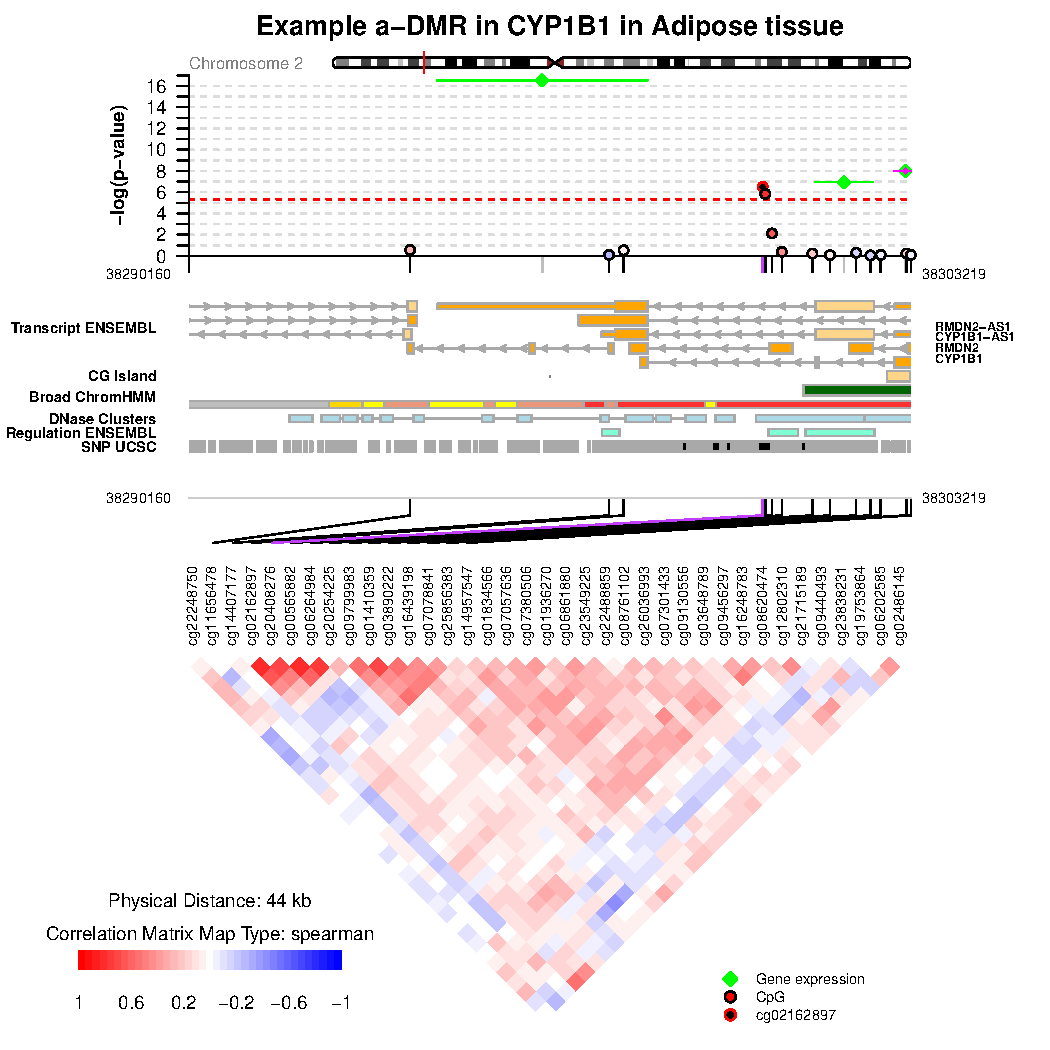
\includegraphics[width=\maxwidth]{figure/minimal-cometwebPlot} 

}



\end{knitrout}
\caption{Plot with comet.web function.\label{fig:cometweb_simple}}
\end{figure}

\section{Creating a plot with the generic function: comet}
It is possible to create the annotation tracks by Gviz, trackviewer or ggbio, for example see Figure \ref{fig:cometPlot}.
Currently, the Gviz option for annotation tracks, in combination with the heatmap of correlation values between genetics elements, provides the most informative and easy approach to visualize graphics.

\subsection{coMET plot: pvalue plot, annotation tracks, and correlation matrix}
\begin{knitrout}
\definecolor{shadecolor}{rgb}{0.969, 0.969, 0.969}\color{fgcolor}\begin{kframe}
\begin{alltt}
\hlstd{extdata} \hlkwb{<-} \hlkwd{system.file}\hlstd{(}\hlstr{"extdata"}\hlstd{,} \hlkwc{package}\hlstd{=}\hlstr{"coMET"}\hlstd{,}\hlkwc{mustWork}\hlstd{=}\hlnum{TRUE}\hlstd{)}
\hlstd{configfile} \hlkwb{<-} \hlkwd{file.path}\hlstd{(extdata,} \hlstr{"config_cyp1b1_zoom_4comet.txt"}\hlstd{)}
\hlstd{myinfofile} \hlkwb{<-} \hlkwd{file.path}\hlstd{(extdata,} \hlstr{"cyp1b1_infofile.txt"}\hlstd{)}
\hlstd{myexpressfile} \hlkwb{<-} \hlkwd{file.path}\hlstd{(extdata,} \hlstr{"cyp1b1_infofile_exprGene_region.txt"}\hlstd{)}
\hlstd{mycorrelation} \hlkwb{<-} \hlkwd{file.path}\hlstd{(extdata,} \hlstr{"cyp1b1_res37_rawMatrix.txt"}\hlstd{)}

\hlstd{chrom} \hlkwb{<-} \hlstr{"chr2"}
\hlstd{start} \hlkwb{<-} \hlnum{38290160}
\hlstd{end} \hlkwb{<-} \hlnum{38303219}
\hlstd{gen} \hlkwb{<-} \hlstr{"hg19"}
\hlstd{strant} \hlkwb{<-} \hlstr{"*"}

\hlstd{BROWSER.SESSION}\hlkwb{=}\hlstr{"UCSC"}
\hlstd{mySession} \hlkwb{<-} \hlkwd{browserSession}\hlstd{(BROWSER.SESSION)}
\hlkwd{genome}\hlstd{(mySession)} \hlkwb{<-} \hlstd{gen}

\hlstd{genetrack} \hlkwb{<-}\hlkwd{genesENSEMBL}\hlstd{(gen,chrom,start,end,}\hlkwc{showId}\hlstd{=}\hlnum{FALSE}\hlstd{)}
\hlstd{snptrack} \hlkwb{<-} \hlkwd{snpBiomart}\hlstd{(chrom, start, end,} \hlkwc{dataset}\hlstd{=}\hlstr{"hsapiens_snp_som"}\hlstd{,}\hlkwc{showId}\hlstd{=}\hlnum{FALSE}\hlstd{)}
\hlstd{strutrack} \hlkwb{<-} \hlkwd{structureBiomart}\hlstd{(chrom, start, end, strand,}
                              \hlkwc{dataset}\hlstd{=}\hlstr{"hsapiens_structvar_som"}\hlstd{,}\hlkwc{showId}\hlstd{=}\hlnum{FALSE}\hlstd{)}
\hlstd{iscatrack} \hlkwb{<-}\hlkwd{ISCATrack}\hlstd{(gen,chrom,start,end,mySession,} \hlkwc{table}\hlstd{=}\hlstr{"iscaPathogenic"}\hlstd{)}

\hlstd{listgviz} \hlkwb{<-} \hlkwd{list}\hlstd{(genetrack,snptrack,iscatrack)}


\hlkwd{comet}\hlstd{(}\hlkwc{config.file}\hlstd{=configfile,} \hlkwc{MYDATA.FILE}\hlstd{=myinfofile,} \hlkwc{CORMATRIX.FILE}\hlstd{=mycorrelation,}
      \hlkwc{MYDATA.LARGE.FILE}\hlstd{=myexpressfile,} \hlkwc{TRACKS.GVIZ}\hlstd{=listgviz,}
      \hlkwc{VERBOSE}\hlstd{=}\hlnum{FALSE}\hlstd{,} \hlkwc{PRINT.IMAGE}\hlstd{=}\hlnum{FALSE}\hlstd{)}
\end{alltt}
\end{kframe}
\end{knitrout}

\begin{figure}
\begin{knitrout}
\definecolor{shadecolor}{rgb}{0.969, 0.969, 0.969}\color{fgcolor}

{\centering 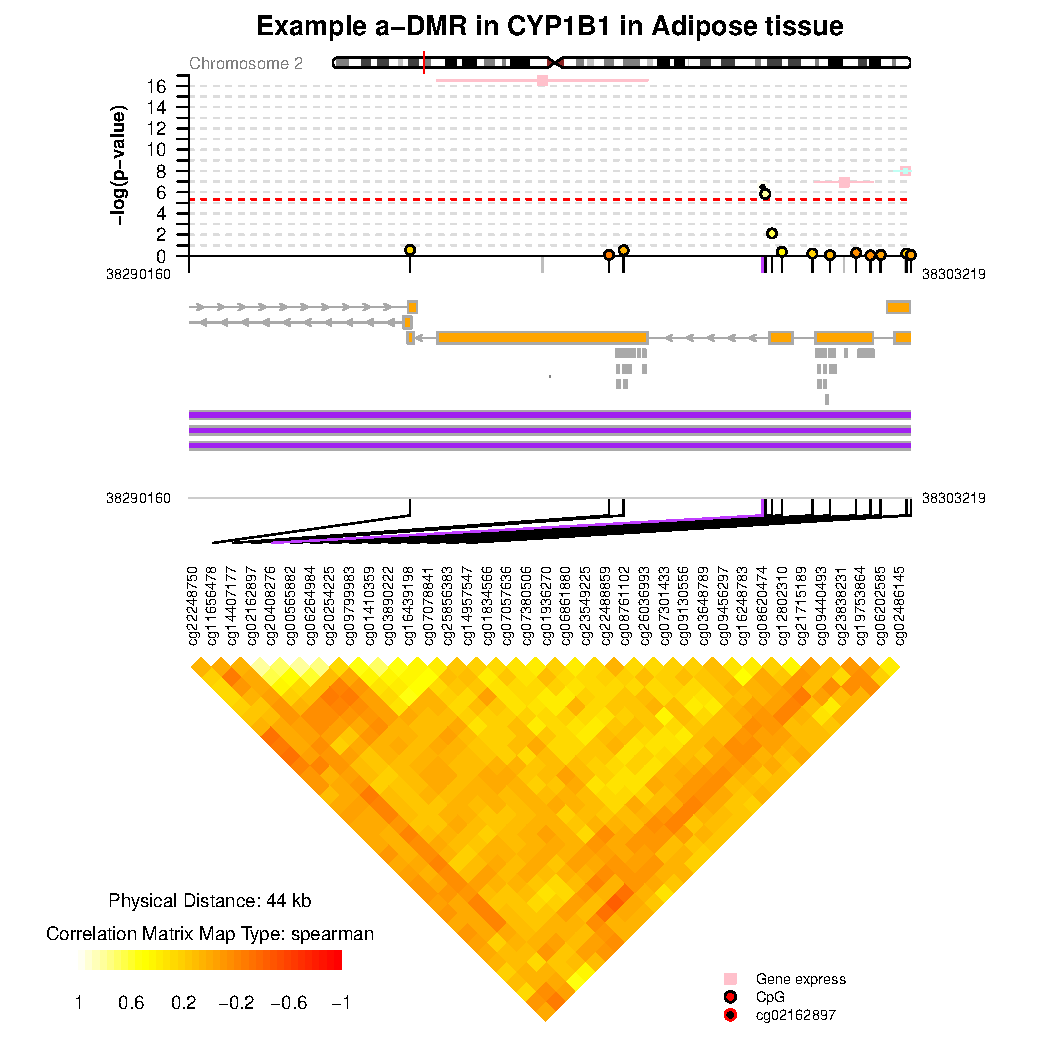
\includegraphics[width=\maxwidth]{figure/minimal-cometPlot} 

}



\end{knitrout}
\caption{Plot with comet function.\label{fig:cometPlot}}
\end{figure}

\subsection{coMET plot: annotation tracks and correlation matrix}  
It is possible to visualise only annotation tracks and the correlation between genetic elements.
In this case, we need to use the option \texttt{DISP.PVALUEPLOT=FALSE}, for example see Figure \ref{fig:cometPlot_nopval}.

\begin{knitrout}
\definecolor{shadecolor}{rgb}{0.969, 0.969, 0.969}\color{fgcolor}\begin{kframe}
\begin{alltt}
\hlstd{extdata} \hlkwb{<-} \hlkwd{system.file}\hlstd{(}\hlstr{"extdata"}\hlstd{,} \hlkwc{package}\hlstd{=}\hlstr{"coMET"}\hlstd{,}\hlkwc{mustWork}\hlstd{=}\hlnum{TRUE}\hlstd{)}
\hlstd{configfile} \hlkwb{<-} \hlkwd{file.path}\hlstd{(extdata,} \hlstr{"config_cyp1b1_zoom_4cometnopval.txt"}\hlstd{)}
\hlstd{myinfofile} \hlkwb{<-} \hlkwd{file.path}\hlstd{(extdata,} \hlstr{"cyp1b1_infofile.txt"}\hlstd{)}
\hlstd{mycorrelation} \hlkwb{<-} \hlkwd{file.path}\hlstd{(extdata,} \hlstr{"cyp1b1_res37_rawMatrix.txt"}\hlstd{)}
\hlcom{#configfile <- "../inst/extdata/config_cyp1b1_zoom_4comet.txt" }

\hlstd{chrom} \hlkwb{<-} \hlstr{"chr2"}
\hlstd{start} \hlkwb{<-} \hlnum{38290160}
\hlstd{end} \hlkwb{<-} \hlnum{38303219}
\hlstd{gen} \hlkwb{<-} \hlstr{"hg19"}

\hlstd{genetrack} \hlkwb{<-}\hlkwd{genesENSEMBL}\hlstd{(gen,chrom,start,end,}\hlkwc{showId}\hlstd{=}\hlnum{FALSE}\hlstd{)}
\hlstd{snptrack} \hlkwb{<-} \hlkwd{snpBiomart}\hlstd{(chrom, start, end,}
                       \hlkwc{dataset}\hlstd{=}\hlstr{"hsapiens_snp_som"}\hlstd{,}\hlkwc{showId}\hlstd{=}\hlnum{FALSE}\hlstd{)}
\hlstd{strutrack} \hlkwb{<-} \hlkwd{structureBiomart}\hlstd{(chrom, start, end,}
                              \hlstd{strand,} \hlkwc{dataset}\hlstd{=}\hlstr{"hsapiens_structvar_som"}\hlstd{)}
\hlstd{clinVariant}\hlkwb{<-}\hlkwd{ClinVarMainTrack}\hlstd{(gen,chrom,start,end)}
\hlstd{clinCNV}\hlkwb{<-}\hlkwd{ClinVarCnvTrack}\hlstd{(gen,chrom,start,end)}
\hlstd{gwastrack} \hlkwb{<-}\hlkwd{GWASTrack}\hlstd{(gen,chrom,start,end)}
\hlstd{geneRtrack} \hlkwb{<-}\hlkwd{GeneReviewsTrack}\hlstd{(gen,chrom,start,end)}

\hlstd{listgviz} \hlkwb{<-} \hlkwd{list}\hlstd{(genetrack,snptrack,strutrack,clinVariant,}
                 \hlstd{clinCNV,gwastrack,geneRtrack)}
\hlkwd{comet}\hlstd{(}\hlkwc{config.file}\hlstd{=configfile,} \hlkwc{MYDATA.FILE}\hlstd{=myinfofile,} \hlkwc{CORMATRIX.FILE}\hlstd{=mycorrelation,}
      \hlkwc{TRACKS.GVIZ}\hlstd{=listgviz,} \hlkwc{VERBOSE}\hlstd{=}\hlnum{FALSE}\hlstd{,} \hlkwc{PRINT.IMAGE}\hlstd{=}\hlnum{FALSE}\hlstd{,}\hlkwc{DISP.PVALUEPLOT}\hlstd{=}\hlnum{FALSE}\hlstd{)}
\end{alltt}
\end{kframe}
\end{knitrout}

\begin{figure}
\begin{knitrout}
\definecolor{shadecolor}{rgb}{0.969, 0.969, 0.969}\color{fgcolor}

{\centering 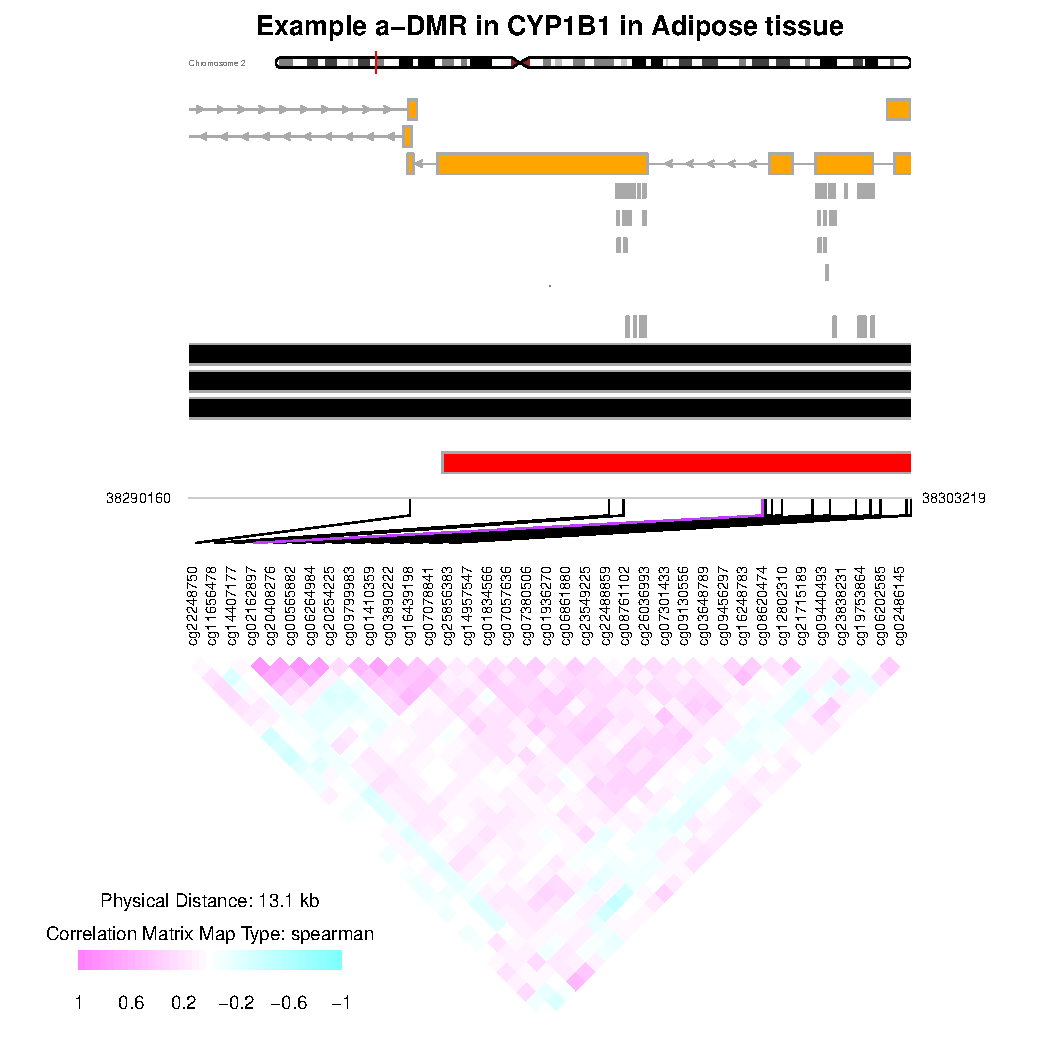
\includegraphics[width=\maxwidth]{figure/minimal-cometPlot_nopval} 

}



\end{knitrout}
\caption{Plot with comet function without pvalue plot.\label{fig:cometPlot_nopval}}
\end{figure}


\clearpage
\section*{SessionInfo}
The following is the session info that generated this vignette:
\begin{kframe}
\begin{alltt}
\hlkwd{toLatex}\hlstd{(}\hlkwd{sessionInfo}\hlstd{())}
\end{alltt}
\end{kframe}\begin{itemize}\raggedright
  \item R version 3.1.1 (2014-07-10), \verb|x86_64-pc-linux-gnu|
  \item Locale: \verb|LC_CTYPE=en_GB.UTF-8|, \verb|LC_NUMERIC=C|, \verb|LC_TIME=en_US.UTF-8|, \verb|LC_COLLATE=en_GB.UTF-8|, \verb|LC_MONETARY=en_US.UTF-8|, \verb|LC_MESSAGES=en_GB.UTF-8|, \verb|LC_PAPER=en_US.UTF-8|, \verb|LC_NAME=C|, \verb|LC_ADDRESS=C|, \verb|LC_TELEPHONE=C|, \verb|LC_MEASUREMENT=en_US.UTF-8|, \verb|LC_IDENTIFICATION=C|
  \item Base packages: base, datasets, graphics, grDevices, grid, methods,
    parallel, stats, utils
  \item Other packages: BiocGenerics~0.10.0, biomaRt~2.20.0, coMET~0.99.3,
    GenomeInfoDb~1.0.2, GenomicRanges~1.16.4, Gviz~1.8.4, IRanges~1.22.10,
    knitr~1.6, rtracklayer~1.24.2, XVector~0.4.0
  \item Loaded via a namespace (and not attached): acepack~1.3-3.3,
    AnnotationDbi~1.26.1, base64enc~0.1-2, BatchJobs~1.4, BBmisc~1.7,
    Biobase~2.24.0, BiocParallel~0.6.1, BiocStyle~1.2.0, Biostrings~2.32.1,
    biovizBase~1.12.3, bitops~1.0-6, brew~1.0-6, BSgenome~1.32.0, checkmate~1.4,
    cluster~1.15.3, codetools~0.2-9, colorspace~1.2-4, colortools~0.1.5,
    DBI~0.3.1, dichromat~2.0-0, digest~0.6.4, evaluate~0.5.5, fail~1.2,
    foreach~1.4.2, foreign~0.8-61, formatR~1.0, Formula~1.1-2,
    GenomicAlignments~1.0.6, GenomicFeatures~1.16.3, ggbio~1.12.10,
    ggplot2~1.0.0, gridExtra~0.9.1, gtable~0.1.2, gWidgets~0.0-54,
    gWidgetstcltk~0.0-55, hash~2.2.6, highr~0.3, Hmisc~3.14-5, iterators~1.0.7,
    lattice~0.20-29, latticeExtra~0.6-26, MASS~7.3-34, matrixStats~0.10.0,
    munsell~0.4.2, nnet~7.3-8, pbapply~1.1-1, plyr~1.8.1, proto~0.3-10,
    RColorBrewer~1.0-5, Rcpp~0.11.3, RCurl~1.95-4.3, reshape2~1.4,
    R.methodsS3~1.6.1, rpart~4.1-8, Rsamtools~1.16.1, RSQLite~0.11.4,
    scales~0.2.4, sendmailR~1.2-1, splines~3.1.1, stats4~3.1.1, stringr~0.6.2,
    survival~2.37-7, tcltk~3.1.1, tools~3.1.1, trackViewer~1.0.2,
    VariantAnnotation~1.10.5, XML~3.98-1.1, zlibbioc~1.10.0
\end{itemize}

\end{document}
